\documentclass{beamer}

\usetheme[]{Rochester}
\usecolortheme{beaver}
\usepackage[latin1]{inputenc}
\usepackage{graphics}

\author{Will Webberley}
\date{Autumn 2014}
\institute[COMSC]{Cardiff School of Computer Science and Informatics}



\title{Human Factors}
\subtitle{CM2101: Human-Computer Interaction}

\begin{document}

\frame{\titlepage}

\frame{
    \frametitle{Human factors}
    \begin{center}
        ``To design systems that take into account the interaction between them and the people that use them''
    \end{center}
    \begin{itemize}
        \item Multi-disciplinary 
        \begin{itemize}
            \item Biomechanics
            \item Engineering
            \item Psychology
            \item Physiology
            \item ...
        \end{itemize}               
    \end{itemize}
}

\frame{
    \frametitle{Human factors in interaction design}
    \begin{itemize}
        \item Account for human \alert{limitations}
        \item Exploit human \alert{abilities}
        \item Understand everyone is different 
        \item Need to cater for most people in target audience
        \item Address human factors to help improve \alert{usability}
        \vskip20pt
        \item Aim: to improve ability and efficiency in what people do (\alert{ergonomics})
    \end{itemize}
}

\frame{
    \frametitle{Human factors: ergonomics}
    \textbf{Three main types:}
    \vskip20pt
    \begin{itemize}
        \item \alert{Physical} ergonomics
        \vskip10pt
        \item \alert{Cognitive} ergonomics
        \vskip10pt
        \item \alert{Organisational} ergonomics
    \end{itemize}
}

\frame{
    \frametitle{Human factors: Physical ergonomics}
    \begin{itemize}
        \item Limitations/ability of human anatomy 
        \item Concerned with \alert{Perception} and \alert{Execution} in \textit{Gulfs of E \& E}
        \item Consider \alert{physical} human mechanics
        \item Can humans interact sensibly with your hardware interface?
        \item Can they also do so \alert{safely}?
        \begin{itemize}
            \item Repetitive strain injury
            \item People with arthritis
            \item If using for long periods of time, what considerations?
        \end{itemize}
    \end{itemize}
}

\frame{
    \frametitle{Human factors: Physical ergonomics}
    \textbf{Considering hardware displays}
    \begin{columns}
        \column{.7\textwidth}
            \begin{itemize}
                \item Used all day everyday 
                \begin{itemize}
                    \item At work (laptops, desktops)
                    \item At home (tablets, TVs)
                    \item Out \& about (smartphones, smartwatches)
                \end{itemize}
                \item Things need to be clearly \alert{visible}
                \item This helps usability
                \item This also helps reduce eye strain
            \end{itemize}
        \column{.4\textwidth}
            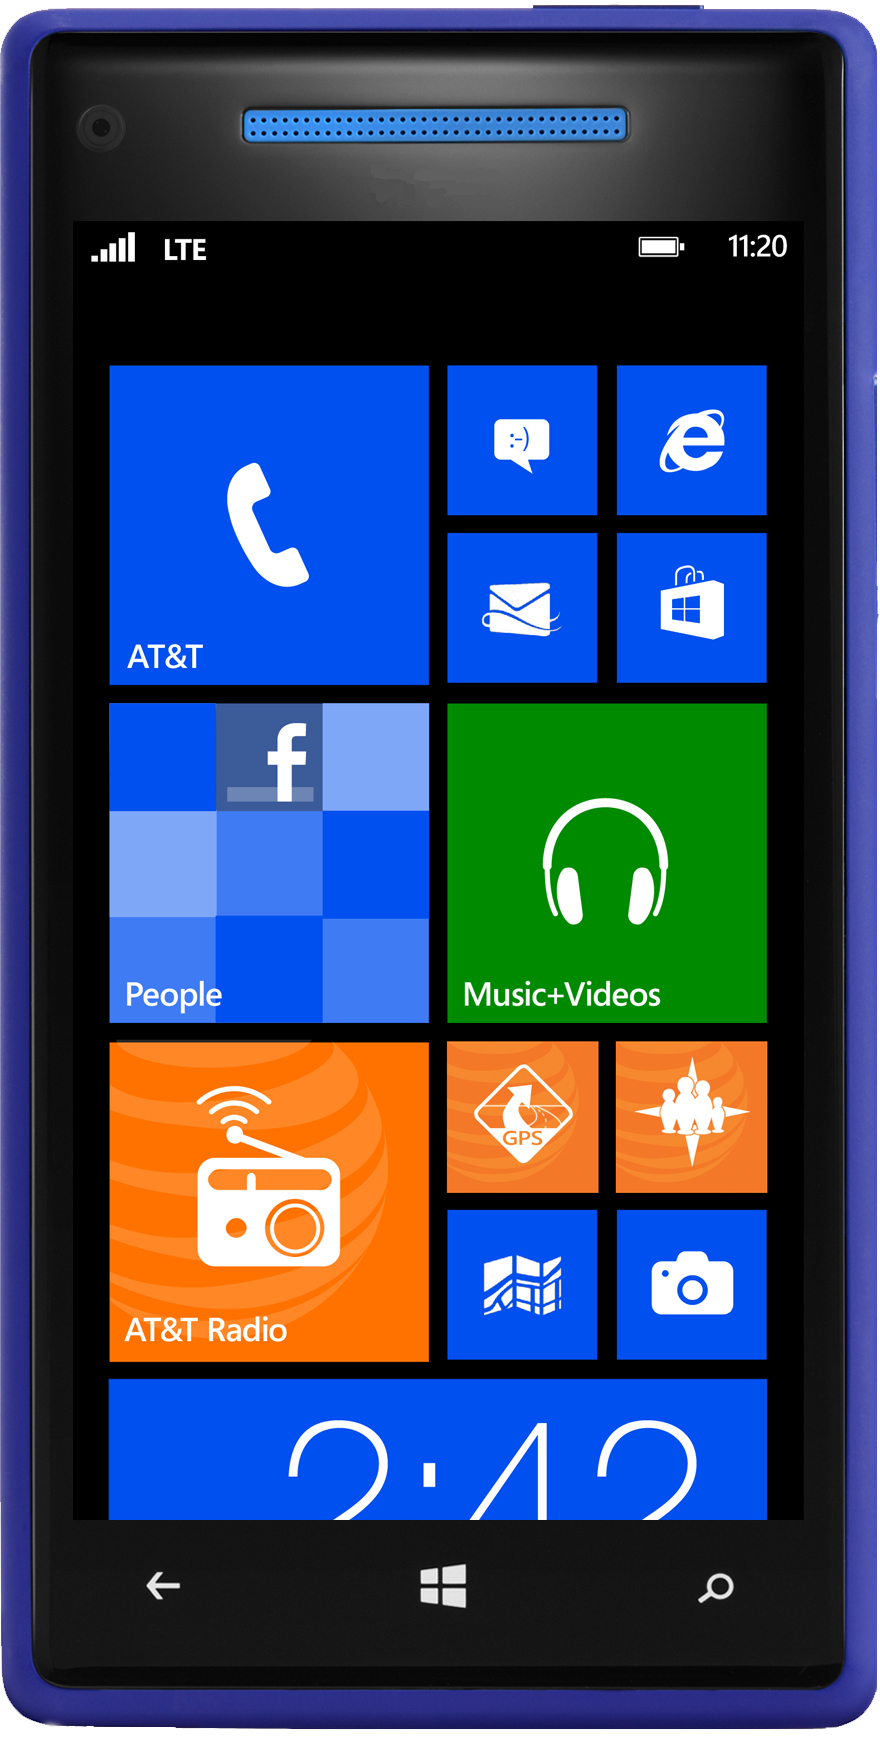
\includegraphics[width=3cm]{media/wp8.jpg}
    \end{columns}
}

\frame{
    \frametitle{Human factors: Physical ergonomics}
    \textbf{Colour perception in humans}
    \begin{itemize}
        \item Human eye able to distuinguish 7,000,000 shades of colour
        \item However, contrast is important to reduce eye strain and improve usability
        \item Also, using a smaller palette improves \alert{Consistency}
        \item Other factors to consider: colour-blindedness, age, place of use
    \end{itemize}
}

\frame{
    \frametitle{Human factors: Physical ergonomics}
    \textbf{Colour-blindedness}
    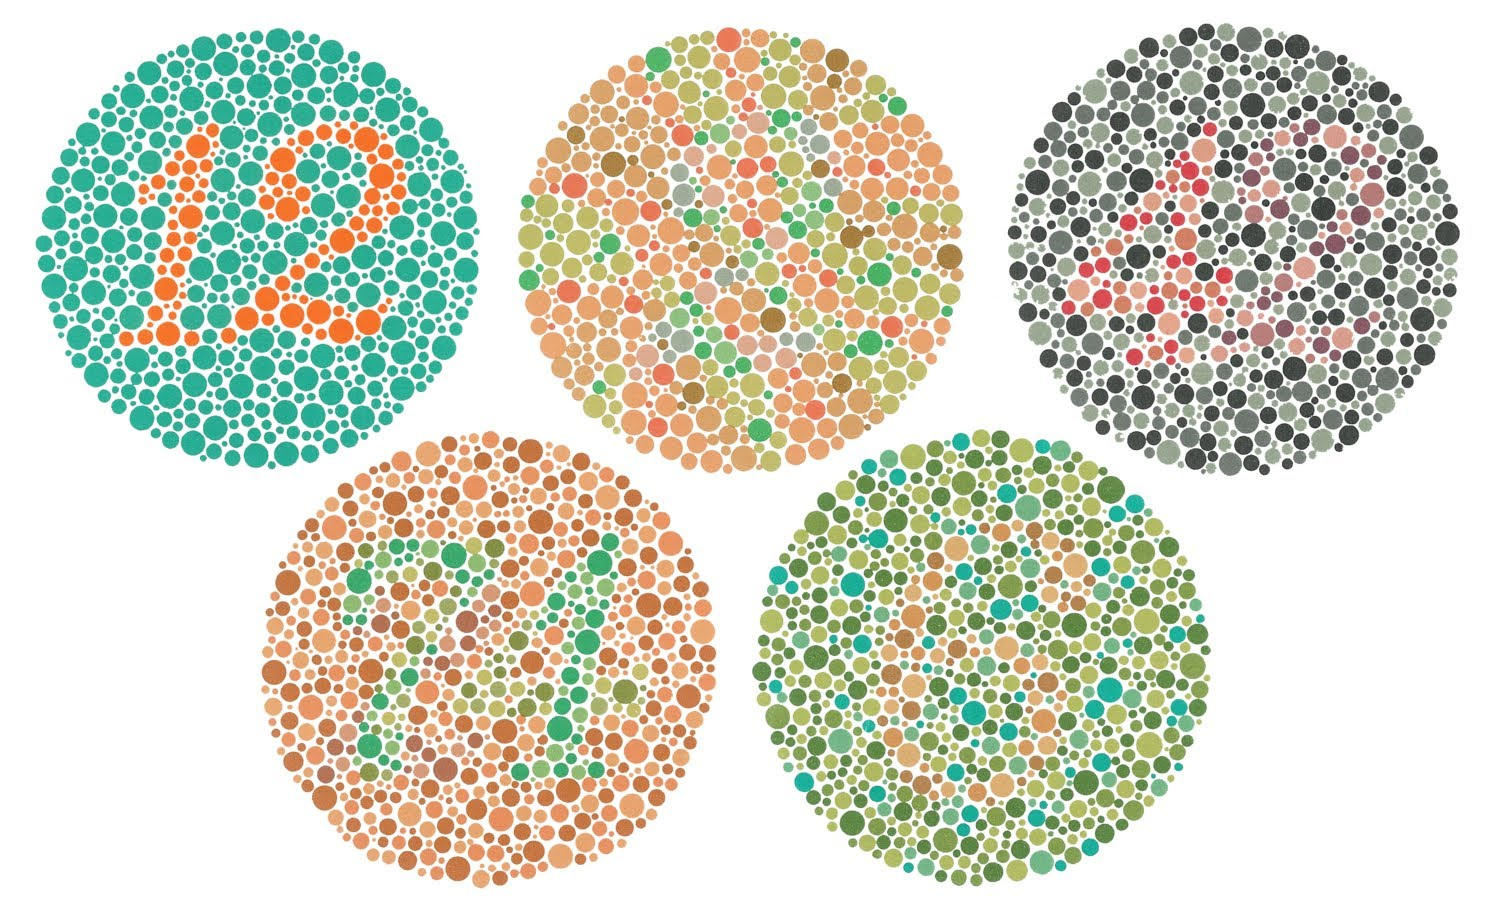
\includegraphics[width=\textwidth]{media/colour_blind_test.jpg}
}

\frame{
    \frametitle{Human factors: Physical ergonomics}
    \textbf{Colour-blindedness}
    \begin{columns}
        \column{.6\textwidth}
            \begin{itemize}
                \item Only affects a small proportion...
                \item ... But likely to exist in most demographics (audiences)
                \vskip20pt
                \item Protanopia \& deuteranopia
                \begin{itemize}
                    \item 8\% of males
                    \item 0.5\% of females
                \end{itemize}
                \item Tritanopia
                \begin{itemize}
                    \item About 50 in a million
                \end{itemize}
            \end{itemize}
        \column{.5\textwidth}
            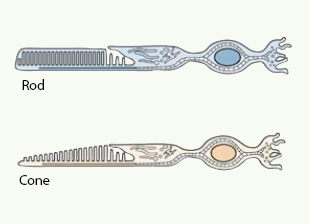
\includegraphics[width=5cm]{media/rod_cone.jpg}
    \end{columns}
}

\frame{
    \frametitle{Human factors: Physical ergonomics}
    \textbf{Age-related factors}
    \begin{columns}
        \column{.5\textwidth}
            \begin{itemize}
                \item Lens loses elasticity
                \begin{itemize}
                    \item Harder to see close things
                \end{itemize}
                \item Yellowing of lens absorbs shortwave light
                \begin{itemize}
                    \item Blue colours harder to focus on
                \end{itemize}
                \item Pupil shrinks, so less light reaches retina
                \begin{itemize}
                    \item Low-contrasting colours harder to view
                \end{itemize}
            \end{itemize}
        \column{.5\textwidth}
            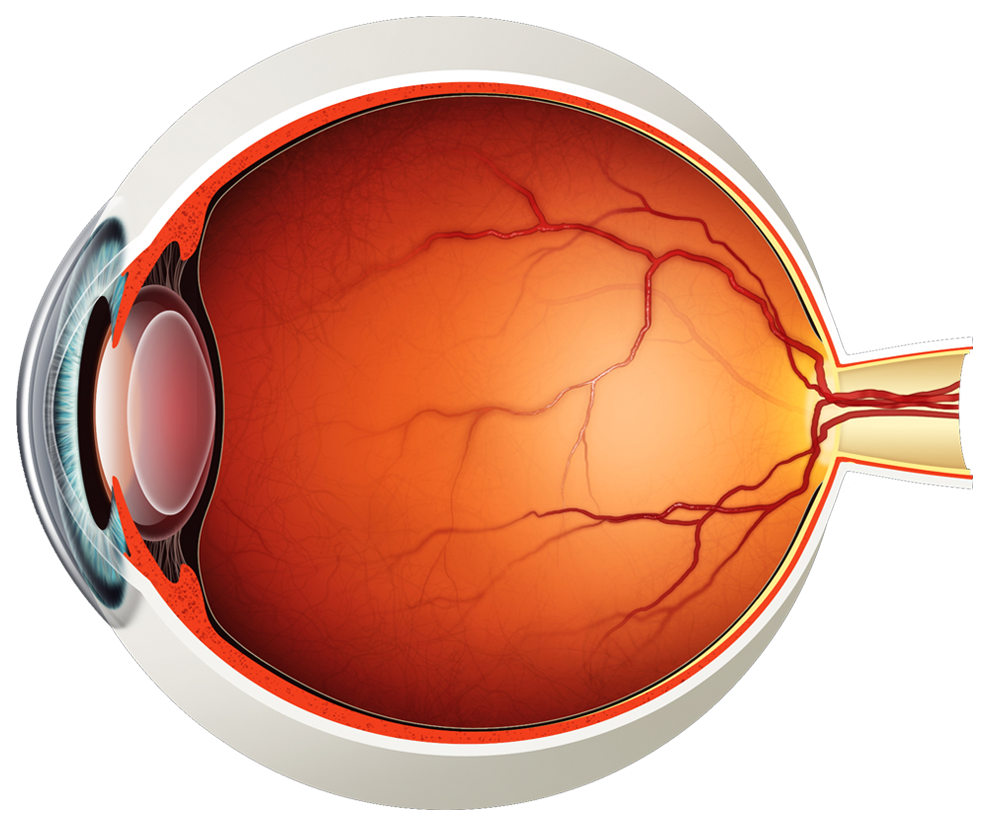
\includegraphics[width=5cm]{media/eye.png}
    \end{columns}
}

\frame{
    \frametitle{Human factors: Physical ergonomics}
    \textbf{The Stroop Effect}  
    \vskip10pt
    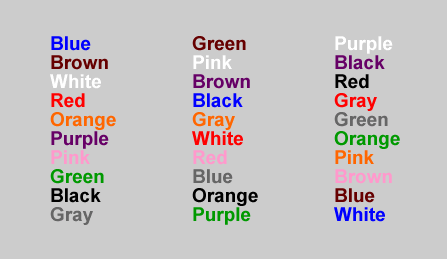
\includegraphics[width=\textwidth]{media/stroop.png}
}

\frame{
    \frametitle{Human factors: Physical ergonomics}
    \textbf{Therefore, some general guidelines:}
    \begin{itemize}
        \item Consider colour-blindedness
        \begin{itemize}
            \item Avoid using red and green together (e.g. red text on greeen BG)
            \item Don't rely solely on colour (use icons, shapes, location to indicate functions)
        \end{itemize}
        \item Consider age
        \begin{itemize} 
            \item Don't use pure blue for text, lines, symbols
            \item Ensure greater contrast and brightness levels
            \item Put important things in centre of screen (not in periphery)
        \end{itemize}
        \item Consider visio-cognitive effects
        \begin{itemize}
            \item Make visual \alert{perception} equal visual \alert{meaning}
            \item Interference in gulf of evaluation causes slow response time
            \item Also consider conflict (e.g. red for `go')
        \end{itemize}
    \end{itemize}
}

\frame{
    \frametitle{Human factors: Physical ergonomics}
    \begin{center}
        Also consider other physical factors (such as movement, tactile senses, etc.), but visual factors are main focus for displays.
    \end{center}
    \vskip30pt
    There are useful tools for finding colours:
    \begin{itemize}
        \item Useful JS lib for colour palettes: \alert{please.js} 
        \item Web services, such as the crowdsourced \alert{color.adobe.com}
    \end{itemize}
}

\frame{
    \frametitle{Human factors: Cognitive ergonomics}
    \begin{itemize}
        \item Limitiation/ability of human mind
        \item Concerned with \alert{Evaluation} and \alert{Planning} in \textit{Gulfs of E \& E}
        \item Can humans \alert{understand} what the interface is telling them?
        \item Can humans make \alert{decisions} based on what the interface allows?
        \item Having \textit{seen} information, can we \textit{understand} it?
        \item With a goal in mind, can we work out \textit{how} to achieve it?
    \end{itemize}
}

\frame{
    \frametitle{Human factors: Cognitive ergonomics}
    \textbf{Considering effective page/screen layout}
    \begin{itemize}
        \item To manipulate attention to convey
        \begin{itemize}
            \item Meaning
            \item Sequence
            \item Areas of interaction
        \end{itemize}
        \item For effective page layout, consider:
        \begin{itemize}
            \item Visual \alert{hierarchy}
            \item Visual \alert{flow}
            \item \alert{Focal} point
        \end{itemize}
    \end{itemize}
}

\frame{
    \frametitle{Human factors: Cognitive ergonomics}
    \textbf{Gestalt laws of grouping for screen layout}
    \vskip20pt
    \begin{columns}
        \column{.5\textwidth}
            \alert{Law of proximity}
            \vskip20pt
            \begin{itemize}
                \item Stimuli close together perceived as one object
                \item Distant stimuli are different objects
                \item Allows for clustering into sets
            \end{itemize}
        \column{.5\textwidth}
            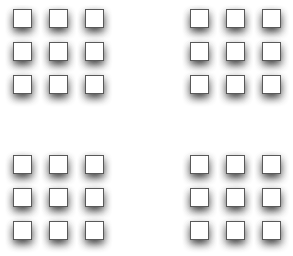
\includegraphics[width=5cm]{media/proximity.png}
    \end{columns} 
}

\frame{
    \frametitle{Human factors: Cognitive ergonomics}
    \textbf{Gestalt laws of grouping for screen layout}
    \vskip20pt
    \begin{columns}
        \column{.5\textwidth}
            \alert{Law of continuity}
            \vskip20pt
            \begin{itemize}
                \item Objects with intersection pereceived as one object
                \item Objects arranged on smooth curve perceived as unit 
            \end{itemize}
        \column{.5\textwidth}
            
\includegraphics[width=5cm]{media/continuity.png}
    \end{columns} 
}

\frame{
    \frametitle{Human factors: Cognitive ergonomics}
    \textbf{Gestalt laws of grouping for screen layout}
    \vskip20pt
    \begin{columns}
        \column{.5\textwidth}
            \alert{Law of closure}
            \vskip20pt
            \begin{itemize}
                \item Perceive as complete even if incomplete
                \item Humans recognise familiar patterns and `fill in the gaps'
                \item e.g. if shape border missing, humans can still perceive the shape
            \end{itemize}
        \column{.3\textwidth}
            
\includegraphics[width=3cm]{media/closure.png}
    \end{columns} 
}

\frame{
    \frametitle{Human factors: Cognitive ergonomics}
    \textbf{Gestalt laws of grouping for screen layout}
    \vskip20pt
    \begin{columns}
        \column{.5\textwidth}
            \alert{Law of similarity}
            \vskip20pt
            \begin{itemize}
                \item Similar stimuli perceived as one object
                \item Different stimuli are a different object
                \item Again, allows for clustering into sets 
            \end{itemize}
        \column{.5\textwidth}
            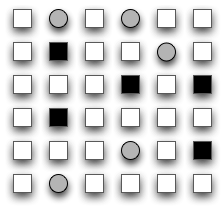
\includegraphics[width=5cm]{media/similarity.png}
    \end{columns} 
}

\frame{
    \frametitle{Human factors: Cognitive ergonomics}
    \textbf{Gestalt laws of grouping for screen layout}
    \vskip20pt
    \alert{Apply together, where possible}
    \vskip20pt
    \begin{itemize}
        \item \alert{Combine} the principles
        \item Helps in understanding what the interface is trying to \alert{say}
        \item Helps humans identify possible \alert{actions}
        \item Helps humans understand what actions might \alert{do}
    \end{itemize}
}

\frame{
    \frametitle{Human factors: Cognitive ergonomics}
    \textbf{Example: \alert{similarity} \& \alert{continuity}}
    \vskip30pt
    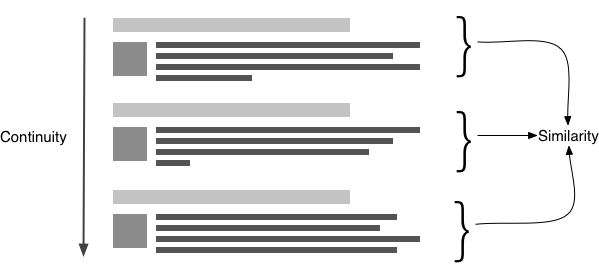
\includegraphics[width=\textwidth]{media/similarity_continuity.png}
}

\frame{
    \frametitle{Human factors: Cognitive ergonomics}
    \textbf{Example: \alert{proximity} \& \alert{closure}}
    \vskip30pt
    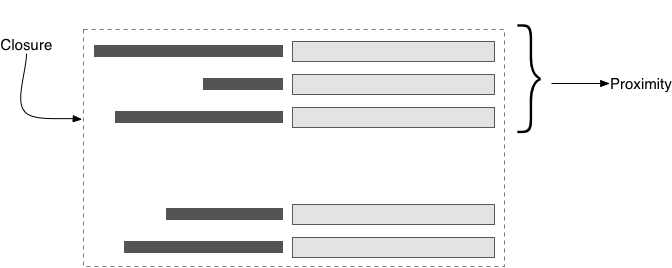
\includegraphics[width=\textwidth]{media/proximity_closure.png}
}

\frame{
    \frametitle{Human factors: Organisational ergonomics}
    \begin{itemize}
        \item Socio-logical aspects of systems
        \item Domain-specific systems
        \item Cultural factors
        \item Organisational guidelines/protocols
    \end{itemize}
}

\frame{
    \frametitle{Human factors: Organisational ergonomics}
    \textbf{Addressing cultural ergonomics}
    \begin{itemize}
        \item Use appropriate wording/imagery
        \begin{itemize}
            \item If designing for hospitals, what acronyms/words do clinicians understand?
            \item If designing for general use, don't use domain-specific terms 
        \end{itemize}   
        \item Use appropriate colours
        \begin{itemize}
            \item Refer to cultural constraints in target audience
            \item Does `red' mean the same in every culture?
        \end{itemize}
    \end{itemize} 
}

\frame{
    \frametitle{Human factors: Organisational ergonomics}
    \begin{center}
        \begin{tabular}{| l | l || r | r |}
            \hline
            \textbf{Colour} & \textbf{Conecpt} & \textbf{American (\%)} & \textbf{Chinese (HK) (\%)}\\
            \hline
            \hline
            Green & Safe & 61.4 & 62.2\\
            Green & Go & 99.2 & 44.7\\
            Red & Hot & 94.5 & 31.1\\
            Red & Danger & 89.9 & 64.7\\
            Red & Stop & 100.0 & 48.5\\
            Yellow & Caution & 81.1 & 44.8\\
            \hline
        \end{tabular}
    \end{center}
}

\frame{
     \frametitle{Revision questions}
     \begin{enumerate}
        \item What are human factors in the context of interaction design?
        \item What is the point of considering human factors?
        \item Describe how considering human factors could address the Gulfs of Evaluation and Execution.
        \item Why is the human visual system important to consider?
        \item What is meant by cognitive ergonimics?
        \item Describe how cognitive ergonomics can be addressed in interaction design.
     \end{enumerate}
}

\frame{
    \frametitle{Summary}
    \begin{itemize}
        \item Human factors in interaction design
        \item Physical ergonomics human factors
        \begin{itemize}
            \item Human visual system
        \end{itemize}
        \item Cognitive ergonomics human factors
        \begin{itemize}
            \item Gestalt principles
        \end{itemize}
        \item Organisational ergonomics human factors
    \end{itemize}
}    

\end{document}
